\documentclass[a4paper,12pt]{article}
\usepackage{caption}
\usepackage{graphicx}
\graphicspath{ {img/} }
\usepackage{fancyhdr}
\pagestyle{fancy}
\lhead{tqvj24}
\chead{}
\rhead{Image Processing Assignment}

\begin{document}

\section*{Discussion/detail of system design and choices made (5\%)}
\subsection*{System Design}
I wrote this script using Python 3.5.2, and OpenCv 3.1.0, to match the versions available on the DUDE PCs in the School.
Operation of the script is done via key presses, and output of the program is both visual in the main window, as well as various images being saved to disk, in the img\_out/ directory.
The main window displays one file ID at a time, with the top row being the w1 channel, and the bottom being w2. These are labelled, and labelling can be toggled by pressing the l key.
Full list of commands:
\begin{itemize}
    \item n - next image
    \item b - previous image
    \item l - toggle labels
    \item s - save the currently displayed w1 and w2 processed images
    \item x - exit
\end{itemize}
There are also boolean settings toward the top of the script, to allow for automatic saving of various images. \\
Processing of images is done in steps, with each step being a standalone method. All methods are documented and commented.
\begin{description}
    \item[Step 1 - Isolate] Isolate the worms
    % TODO from here
\end{description}
% modular processing, in steps, individual methods
% explain each step? With examples under 'evidence' section

\subsection*{Choices Made}
% bit shifting before converting to 8bit for more detail
% removing border via dialation (biggest contour didn't work because of clusters)
% threshold vs histogram equilisation
% comparison to ground truth (very high percentages because of big borders and empty spaces)
% detecting if dead or alive (isContourConvex was bad)

\section*{Evidence of the success of system in performing the specified task (5\%)}
\subsection*{Processing Steps}
% include images here of each step
% 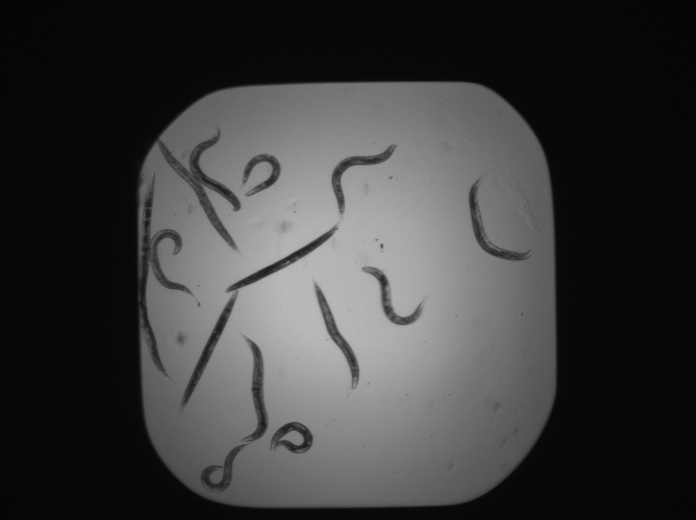
\includegraphics[width=0.95\textwidth]{A01_step0.jpg}  % for example

\centering{tqvj24}
\end{document}
